\documentclass {article}

\title {Geospatial analysis in Scala}
\date {October 2017}

\usepackage {amsmath}
\usepackage {graphicx}
\usepackage {verbatim}
\usepackage {cite}
\usepackage {booktabs}
\usepackage {float}
\usepackage [titletoc, toc, title] {appendix}
\usepackage {hyperref}
\usepackage [T1]{fontenc}

\author {Roxana Tesileanu \\
\\
\href{mailto: roxana.te@web.de}{roxana.te@web.de} \\
INCDS, Romania}

\begin {document}
	\maketitle
	\pagenumbering{gobble}
\tableofcontents

\newpage
\pagenumbering {arabic}
\section {Introduction}

The aim of the present paper is to investigate how the Geospatial Data Abstraction Library (GDAL) \cite{osgeo_gdal_nodate} can be used in Scala \cite{epfl_scala_2017}, for performing the main geospatial analysis tasks: manipulating vector and raster data (geoprocessing) and geospatial data analysis.
  
\subsection {Geoprocessing using GDAL}

Using a programming language for geospatial analysis allows you to customize your analyses instead of being limited to what the software user interface allows.
 This is one of the most important advantages of open source software \cite{garrard_geoprocessing_2016}.
This work uses the GDAL open source library \cite{osgeo_gdal_nodate} developed at the Open Source Geospatial Foundation (OSGeo) (\href{www.osgeo.org}{www.osgeo.org}), and, the Scala programming language developed at \'Ecole polytechnique f\'ed\'erale de Lausanne (EPFL) (\href{http://www.scala-lang.org/}{http://www.scala-lang.org/}) to perform geospatial data analyses. GDAL was written in C and C++ and has bindings for several languages (Java, Perl and Python) \cite{garrard_geoprocessing_2016}.  
\\
\\
In order to use GDAL, you need to install it on your machine, and for its import in Scala you need to install its Java bindings along with it.  
For installation details you can look at the GDAL homepage \href{http://www.gdal.org/}{http://www.gdal.org/}, download GDAL and follow the instructions for building from source, which might not be an easy task, depending on your operating system. 
Thanks to the efforts of the UbuntuGIS team (\href{https://wiki.ubuntu.com/UbuntuGIS}{https://wiki.ubuntu.com/UbuntuGIS}), on Ubuntu, the installation procedure of GDAL and its bindings is done rapidly. Firstly, you need to add the ubuntugis PPA, which offers the official stable UbuntuGIS packages, to your system (\href{https://launchpad.net/~ubuntugis/+archive/ubuntu/ppa}{https://launchpad.net/~ubuntugis/+archive/ubuntu/ppa}). This is done with the commands: \\
\\
sudo add-apt-repository ppa:ubuntugis/ppa \\
sudo apt-get update.\\
\\
Next, you install GDAL on your machine with the commands \cite{safavi_installing_2015} \cite{canonical_ubuntugis_nodate} (\href{http://www.sarasafavi.com/installing-gdalogr-on-ubuntu.html}{http://www\\.sarasafavi.com/installing-gdalogr-on-ubuntu.html}, \href{https://packages.ubuntu.com/source/trusty/gdal}{https://packages.ubuntu.co\\m/source/trusty/gdal}):\\
\\
sudo apt-get install libproj-dev, gdal-bin, libgdal-dev, libgdal-doc \\
sudo apt-get update.\\
\\
Finally, you add the Java bindings to your GDAL package (\href{https://launchpad.net/ubuntu/+source/proj}{https://launchpad.ne\\ t/ubuntu/+source/proj}):\\
\\
sudo apt-get install libgdal-java, libproj-java.    \\
\\
In order to import GDAL in Scala, you have to add its jar to the project's classpath. An easy way of managing dependencies of a Scala project is to use SBT (\href{http://www.scala-sbt.org/}{http://www.scala-sbt.org/}) \cite{tesileanu_using_2017} \cite{suereth_sbt_2016}. In this way you can take advantage of the most convenient way to place the gdal jar to the project's classpath, namely, to place a copy of it into the lib directory of the Scala project, now that the actual installation has already taken place.
\\
\\
Section 1.2 offers an introduction in SBT and into the software development process of Scala projects in general, in order to get ready to start with Section 2 which will offer a background in geoprocessing: manipulating vector data (reading and writing files of different vector data formats, georeferencing data, performing overlay and proximity analyses) and continuing with manipulating raster data (reading and writing files of different raster data formats, resizing pixels, performing moving window analyses and map algebra). 
Then, in Sections 3, 4, 5 and 6 the main approaches of spatial data analyses will be presented, based on variable- and object-based multivariate analyses.     
\\
\\
\subsection{Overview of the software development process of Scala projects}

This subsection offers an introduction into the software development process of Scala projects pointing to some of the available learning resources.
\\
\\
In order to implement software development projects, one should consider which tools to choose for the different components of the development system, which according to Rehman and Paul (2003) \cite{rehman_linux_2003}are the following:
\begin{itemize}
\item  the hardware platform,
\item  the operating system,
\item  editors,
\item compilers, assemblers and debuggers,
\item  version control system, and,
\item  bug tracking.
\end{itemize} 
For implementing Scala projects, working with the Simple Build Tool (SBT) (\href{http://www.scala-sbt.org}{http://www.scala-sbt.org}) condenses the list of the components of a development system, as it unites different steps in one tool (compiling, building, testing and debugging). Another advantage of using SBT is the opportunity of working interactively in Scala REPL, a tool for evaluating expressions in Scala (\href{https://docs.scala-lang.org/overviews/repl/overview.html}{https://docs.scala-lang.org/overviews/repl/overview.html}) within a SBT session with all dependencies and project classes on the classpath, to develop bits of code which can then be inserted in the editor of choice.
\\
\\  
It is also important to understand that software development "is not just writing code", but rather a more comprehensive process \cite{rehman_linux_2003}. 
Rehman and Paul (2003) describe it as comprising the following steps: requirement gathering, writing functional specifications, creating architecture and design documents, implementation and coding, testing and quality assurance, software release, documentation, and, support and, development and release of new features. 
Each project starts with a requirement analysis which investigates the real-world need of the final product. Which functions should the new software carry in real-world problem solving within the specified domain?
 Further, functional specifications are declared to state the functionality of a software product at an abstract level "defining its input/output behavior". 
On the basis of the functional specifications, an architecture of the product is created. 
The architecture "defines the different components of the product and how they interact with each other", without providing the explicit details on how they should be implemented to reach the desired functionality.
 This happens at the design stage, when design documents are created which define each individual component to the level of functions and procedures.
 Using the design documents and development tools (SBT and editor) the code is then implemented and tested.
 There are more types of testing: unit testing (testing one part or one component of the product using test cases to test functionality of this part of the software), sanity testing to check if all components compile, regression or stress testing to check the long-term behavior of the product when used continuously over a period of time, and functional testing using test cases built on functional specifications.
 If a bug (an anomaly) is found it must be reported and fixed. The documentation includes: technical documentation developed during the development process, technical documentation prepared for technical support staff, and end-user manuals and guides. 
Finally, the last stage of the life cycle of a software development project is the support and release of new versions depending on requirements.       
\\
\\
The present subsection aims at introducing the reader to the tools needed to put in motion the development system of Scala projects on Linux, with emphasis on the Ubuntu distribution.      
The following subsubsections will cover brief introductions in using the VIM editor as an editor for Scala code and using SBT to create and manage Scala projects, also addressing the issue of dependency management.

\subsubsection{Using VIM as an editor for Scala code}

VIM is an editor which can be used from within the Linux command line and can be adapted to support the editing of Scala code by installing the vim-scala package of Derek Wyatt found at \href{https://github.com/derekwyatt/vim-scala}{https://github.com/derekwyatt/vim-scala}. 
Under Linux you can install VIM using the package tools at hand (like e.g. dpkg, apt-get, aptitude, rpm or yum) depending on the installed distribution.
 In Ubuntu the command for installing VIM is:  "\$ sudo apt install vim". Afterwards, you open the command line and launch VIM by typing "\$ vim <ENTER>". The following instructions will make the first VIM session easy to pass through:
\begin{itemize}
\item because VIM starts in command mode you can change to insert mode with the "i" key;
\item to exit insert mode and return to command mode, press the <ESC> key;
\item to write the open file to the hard drive use the command ":w filename" (in command mode) or just ":w" if the file already has a name; 
\item to save the changes type ":" in command mode;
\item to exit VIM type ":wq" to quit and save changes, or ":q!" to discard changes (both in command mode);
\item pressing <ESC> will not just place you in command mode but also cancel an unwanted and partially completed command in command mode.
\end{itemize}
\\
\\
The following paragraphs will help you navigate through the VIM file, and, process text (append, delete, copy, paste, search and replace, edit multiple files and get help). 
\\
\\
To move the cursor you use: "l" (or right arrow), "h" (or left arrow), "j" (meaning going down one line), or "k" (meaning going up one line). 
Moving inside the current line is possible with "0" (to go to the beginning of the current line) and "\$" (to go to the end of the current line). 
To go to the end of the file, i.e. to the last line of the file you use "G" and to go to the beginning of the file, i.e. to the first line you use "gg".
 To go to a specific line you use "numbergg" (for example: 2gg to go the the second line).
\\
\\
When you are in command mode, you can start inserting text by using the "i" key to place you in insert mode, but there are also other commands which can place you in insert mode so that you can start appending text. 
One of them is the "a" key, which lets you append text right at the spot where the cursor is placed, or the "A" key which lets you append text directly at the end of the line.
 You can also use the "o" key to open a line below the current line or "O" to open a line above the current line.
\\ 
\\
You can undo changes by using the "u" key and redo changes the using "<CTRL>r".
\\
\\   
Deleting text in command mode goes with (but not only) the following commands:
\begin{itemize}
\item the "x" key deleted the current character; "3x" will delete the current character and the next two characters
\item the "dd" command deletes the current line; "6 d d" will delete the current line and the next five lines
\item the "dG" command will deleted to the end of the file
\item the "d\$" command will delete to the end of the line
\item the "d0" command will delete to the beginning of the line.
\end{itemize}
The commands based on "d" nut just delete text but also copy it to a paste buffer, which can be later recalled with the "p" command to paste the contents of the buffer after the cursor or the "P" command to paste the contents of the buffer before the cursor.
\\
\\
Cutting, copying and pasting text is done more traditionally with the "y" command (which stands for "yank", i.e. copy). 
To copy the current line you use "yy" ("6yy" means copy the current line and the next five lines). To copy to the end of the line use "y\$" and to the beginning of the line use "y0". You can join lines with "J".
\\
\\
Searching and replacing is done within the line and within the whole file. 
Searching within the line is done with "f" from "find" (for example "fa" will move the cursor to the next occurence of "a"). 
You can also use the substitute command for a line (for example: while in command mode "s:caar/car<ENTER>" means substitute "caar" with "car", and replaces the first occurence of the searched word). 
The ":\#,\#s/big/small/g" replaces "big" with "small" within a range of lines (":" starts the command, "\#" stands for a line number and "g" stands for "global"). 
To search the entire file use "/" followed by the searched word and the <ENTER> key. 
You can go to the next occurrence of the searched word with the "n" (from "next") command. 
To search and replace over the entire file, i.e. globally, you can use the command ":\%s/you/YOU/g" (":" starts the command, "\%s" find and substitute, "g" globally). 
The search can also be done with options. For example entering ":set ic" will allow finding also combinations with capitals. To disable ignoring case enter ":set noic".
 You can also enable the "is" option (with the ":set is" command), which can be disabled with ":set nois".
\\
\\
To edit multiple files you can open them together from the beginning (for example "\$ vim file1, file2, file3) or you open additional files after you started VIM with the command ":e additional\underline{\space}file".
 The command "buffers" displays a list of files under editing.
 You can switch between files with the command ": buffer 1" for example to go to the first file listed by the ":buffers" command, or ":buffer 2" to go to the second file listed by the ":buffers" command.
 To copy content from one file to another you copy with yank, switch with buffer and paste. 
This works only if the files were opened together or with the ":e" command. 
Opening different VIM windows will not allow copying between files in this way. Instead, you have to use <SHIFT><CTRL><C> to copy from one file and <SHIFT><CTRL><V> to paste into another file. The <SHIFT><CTRL><V> command lets you paste text from all kind of sources (from documents, web sites, etc.).
 To insert an entire file into another you can use the ":r other\underline{\space}file\underline{\space}name\underline{\space}to\underline{\space}be\underline{\space}inserted\underline{\space}into\underline{\space}the\underline{\space}current" command, where "r" stands for "retrieving".
\\ 
\\
To select text to paste you can also use the visual mode by typing "v" in command mode and then move the cursor to the end of your selection.
 The selected text will be highlighted. Then press "y" to yank it and then "p" to paste it.
\\
\\
A useful debugging command is the matching parentheses command. You can find out if the corresponding parenthesis or bracket is missing with "\%" by moving the cursor on the first parenthesis or bracket and typing "\%".    
\\
\\
To excute and external command, i.e. a command as if you were in the command line, with the ":! your\underline{\space}command" command.
 For example the ":! ls <ENTER>" command will list the objects of the working directory. 
\\
\\
Finally for getting help in VIM you type ":help <ENTER>".
 To close the help window use ":q". 
To find help on a specific command use ":help some\underline{\space}command", for example type ":help user-manual" to get to the user manual.
 For an interactive tutorial for VIM you can also use the "VIM Tutor" initially created by Pierce and Ware, which can be started in the command line with the command "\$ vimtutor <ENTER>". 
A short introduction in VIM can be also found in Shotts (2009) \cite{shotts_linux_2009}, a lecture which gently introduces readers to the Linux command line in general. 

\subsubsection {Using SBT to create and manage Scala projects}

In Section 1.2.2 the reader will find out how to install SBT and use it to create and manage Scala projects. 
Furthermore, the issue of integrating external (managed) and internal (unmanaged) dependencies and of forking the Java Virtual Machine (JVM) will be discussed.

\paragraph {Installing SBT}

You can use the Scala REPL either directly from within the command-line, initiating a REPL sesssion with the command "\$ scala", or, by launching a SBT-session with the command "\$ sbt" and then from within SBT launch the Scala REPL using the command "> console".
 On Ubuntu you can install the Scala language using the apt command ("\$ sudo apt install scala") with no additional commands.
 Check the package management tool you use to get the same result. You can open the Scala REPL and type in some expressions; to exit type ":q" (VIM is useful after all). 
For guidance, check the book of Jason Swartz "Learning Scala" \cite{swartz_learning_2015} and the book of Mark Lewis "Introduction to Programming and Problem Solving Using Scala" \cite{lewis_introduction_2017}for a great introduction to the Scala language. 
\\
\\
Installing SBT requires a look at the SBT homepage (\href{http://www.scala-sbt.org/}{http://www.scala-sbt.org/}) in order to get the four commands needed to install it using the command line.
 At the time the present document is written the commands for Ubuntu  are:
\\
\\
\$ echo "deb https://dl.bintray.com/sbt/debian /" | sudo tee -a /etc/apt/sources.list.d/sbt.list\\
\\
\\
\$ sudo apt-key adv --keyserver hkp://keyserver.ubuntu.com:80 --recv 2EE0EA64E40A89B84B2DF73499E82A75642AC823\\
\\
\\
\$ sudo apt-get update\\
\\
\\
\$ sudo apt-get install sbt\\
\\
\\
If you are using rpm distributions visit the SBT download page (href{http://www.scala-sbt.org/download.html}{http://www.scala-sbt.org/download.html}) and look for the appropriate installing commands. 
\\
\\
Next, open a Scala REPL session in SBT using the commands introduced at the beginning of this section and type in some expressions.
 You exit the console with ":q" and the command "> exit" gets you out of the SBT and back to the command-line.

\paragraph{Creating a Scala projet}

Now, we will create a Scala project called Scala\underline{\space}Playground in order to continue the playground series of Linux introductions started by William Shotts (2009) in his book "The Linux Command Line". 
\\
\\
Open the terminal with <CTRL-ALT-t>. 
It starts directly in your home directory.
 Next, create a directory called Scala\underline{\space}Playground ("\$ mkdir Scala\underline{\space}Playground <ENTER>"). Check if the directory was created with the command "\$ls <ENTER>" which lists the contents of the directory in which you are placed.
 Further, switch to the Scala\underline{\space}Playground directory ("\$ cd Scala\underline{\space}Playground <ENTER>") and create a part of the inner structure of the current directory by adding another directory called src with its subdirectory main, with its subdirectory scala.
 This is done with the command "\$ mkdir -p src/main/scala" which creates the entire chain of directories. Check it with "\$ls" and "\$cd" commands, return to the Scala\underline{\space}Playground directory with "cd - ". 
\\
\\
Next, in the Scala\underline{\space}Playground directory, create a second directory called project.
 The ls command should print now for the Scala\underline{\space}Playground two contents: project and src.  
\\
\\
The final step in creating the Scala project is to create two files: one directly in the Scala\underline{\space}Playground directory called build.sbt and the second in the Scala\underline{\space}Playground/project directory called build.properties. 
Open VIM when you are in the Scala\underline{\space}playground/project directory and type in:
\\
\\
sbt.version = 0.13.15 
\\
\\
Go in the command mode with <ESC> and save the changes and give the open file a name: ":w build.properties".
 Exit vim with ":q". 
\\
\\
The build.properties file sets the version of SBT.
\\
\\
Next, when you are in the Scala\underline{\space}Playground directory open VIM and edit the basic settings of the Scala project: project name, Scala version used, and the dependencies you need. 
For the moment we will ignore dependencies and create the basic Scala project.
 Type in the file opened in VIM the following two lines:
\\
\\
name := "Scala\underline{\space}Playground"\\
scalaVersion := "2.11.10"
\\
\\
The above two lines are not in Scala, they are in SBT's own language \cite{suereth_sbt_2016}.
Now, get into the command line mode with <ESC> and save the changes and give the file the name build.sbt (":w build.sbt").
 Exit VIM with ":q". 
 You should now have three objects in the Scala\underline{\space}Playground directory: the build.sbt file, the project directory and the src directory. 
\\
\\  
You can now launch SBT while you are in the Scala\underline{\space}Playground directory using the "\$ sbt" command. 
You can see the SBT's output as it uses the information from the two edited files and creates the desired Scala project.
 When the output is finished you get to see the SBT prompt ">".
 The project was created successfully.
 Now, launch the Scala REPL with the command "> console". When the REPL is open you get to see the Scala prompt "scala>". 
You can type in some expressions to see if it works. 
Type ":q" to get back to SBT and "exit" to get back to the command-line. 
\\
\\
You can see that the Scala\underline{\space}Playground directory has gained some additional directories: the Scala\underline{\space}Playground/target directory and the Scala\underline{\space}Playground/project/target directory.
 These are created by SBT when it creates the Scala project, and serve as locations for the output of SBT tasks (e.g. output following compilations or packaging actions).  
\\
\\
In the src/main/scala directory you should place your Scala codes in form of scala files.   

\paragraph{Some basic SBT tasks}

Open SBT. When you see the SBT prompt ">" type in your first SBT command: "help". 
This generates an output which you can use to get further information about SBT and about the configuration of your project (command "about", command "settings"). 
The command "reload" reloads the project in the current directory, which is useful after you've changed the project settings (for example after adding dependencies) or after you've changed or added source files.
 It does the sanity check as it compiles the source files and outputs the errors encountered in the compilation process, accompanied by messages indicating possible reasons. 
It is very often helpful to try to read them in order to debug the code. 
\\
\\ 
The command "tasks" is also listed in the help output.
 The SBT tasks show much of the functions SBT can take over.
 Type in "tasks" and check the default list of SBT tasks:
\begin{itemize} 
\item starting the Scala REPL with the command "console"
\item compiling source files with the command "complile"
\item running an application with the command "run" 
\item testing the code executing all tests
\item and many more.
\end{itemize}
For a detailed introduction in SBT you should check the SBT documentation at \href{http://www.scala-sbt.org/documentation.html}{http://www.scala-sbt.org/documentation.html} and read the book of Joshua Suereth and Matthew Farwell (2016) "SBT in action: the Simple Scala Build Tool". 

\subsubsection {Managing dependencies with SBT}

Depending on the field in which a software developer is active, it is often necessary to use field-specific third-party Scala libraries which offer additional functionality.
 For data analysis, for example, the best known libraries are Spark (\href{http://spark.apache.org/}{http://spark.apache.org/}) which is a general engine for large-scale data processing (see \cite{karau_learning_2015} for an introduction in Spark), ScalaNLP (\href{http://www.scalanlp.org/}{http://www.scalanlp.org/}) which is a suite of Machine Learning and numerical computinng libraries, or Figaro (\href{https://www.cra.com/work/case-studies/figaro}{https://www.cra.com/work/case-studies/figaro}) which is a probabilistic programming language for probabilistic modeling based on Scala (see \cite{pfeffer_practical_2016} for an introduction in Figaro). 
\\
\\
For GUI programming, the best known libraries are Scala.swing (\href{http://www.scala-lang.org/api/2.9.1/scala/swing/package.html}{http://www.scala-lang.org/api/2.9.1/scala/swing/package.html}) which is actually a Scala package but needs to be added to the dependencies list in order to be imported and used in Scala projects, and ScalaFX (http://www.scalafx.org/) which is based on Scala and sits on top of JavaFX \cite{lewis_introduction_2017} (see \cite{lewis_introduction_2017} for a general introduction in Scala and GUI programming using Scala).   
\\
\\
For many software developers, the main reason of using SBT is because it offers an easy management of dependencies from repositories.
 Also the packaging and integration of libraries in form of .jar files into the project is possible.
 Internal libraries in form of .jar files are called unmanaged dependencies and you should place them into the project's lib directory, which should be created inside the project's directory if you intend to use libraries in form of .jar files for a Scala project.
 External libraries are found on repositories and are called managed dependencies, as they are configured in the build definition and downloaded automatically from repositories \cite{noauthor_sbt_2017}.  

\paragraph {Using external Scala libraries}

The first step towards integrating the functionality of these external libraries into our Scala code is to find out their repository coordinates for SBT use.
 One way to find out this piece of information is to search for them in the Maven Repository (\href{https://mvnrepository.com/}{https://mvnrepository.com/}). 
The next step is to add the Maven dependency of the external library to the Scala project \cite{karau_learning_2015}. 
This is done by including an additional setting called "libraryDependencies" in the project's buid.sbt file.
 This setting can take the form of a Sequence for including more than one external library dependency and in general looks like the following:
\\
\\
libraryDependencies ++= Seq( \\
groupID \%\% artifactID \% revision,\\
groupID \%\% artifactID \% revision\\
)\\
\\
\\
where the exact library coordinates are found in the Maven Repository.
\\
\\
Figure \ref{fig: fig1} presents the contents of the build.sbt file of a Scala project called Scala\underline{\space}Playground (created in section 3.2) which includes the managed dependencies for enabling the use of Spark's MLlib (Spark's library for Machine Learning) and of scalaFX (library for GUI programming) and, the unmanaged dependecy for enabling the use of javaFX package needed for GUI programming using scalaFX.          
\\
\\
\begin{figure} [H]
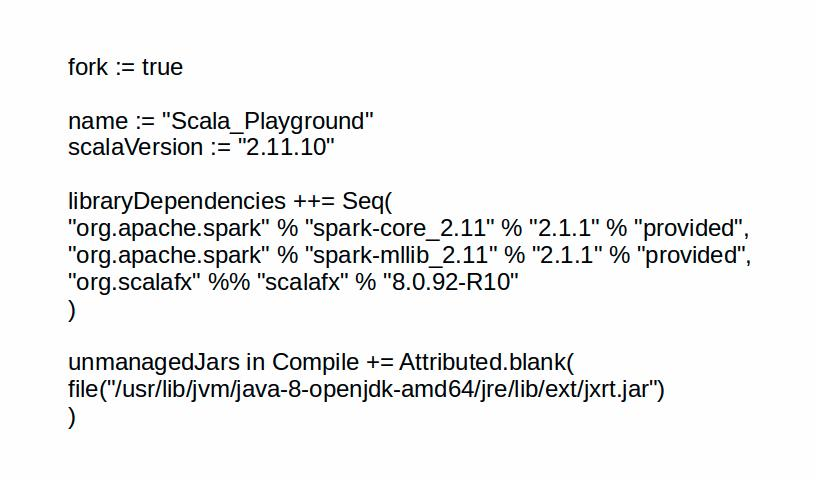
\includegraphics[width=\linewidth] {fig1.jpg}
\caption{The contents of the build.sbt file of a Scala project with three external dependencies and one internal dependency (if more than one .jar file is needed, then they should be placed in the project's lib directory instead of specifying them in the build.sbt file).}
\label{fig: fig1}
\end{figure}   
\\
\\
\paragraph{Using internal Scala libraries}

Sometimes it is necessary to use internal libraries in form of .jar files.
 Jar files are automatically created from compiled source files by setting the variable "exportJars" of the build.sbt file to true (exportJars := true).
 The process of .jar creation is called packaging.
 The newly created .jar file is placed in the project's target/scala-2.11 directory.
 If you want to make use of an internal library in form of a .jar file in your Scala code, it has to be added to classpath so that it becomes available during compilation, testing, running, and when using Scala REPL (\cite{noauthor_sbt_2017}). 
This can be achieved by overriding the settings variable called "unmanaged Jars" and indicating the path to the .jar file you want to use:
\\
\\
unmanagedJars in Compile := Attributed.blank(file("mypath/*.jar")). 
\\
\\
The above setting is equivalent to the use of "-cp" when starting the Scala interpreter from outside SBT ("\$ scala - cp mypath/*.jar ").      
\\
\\
If more than one .jar file is used, then you should create a new directory called lib inside the Scala project's directory in which you can place the necessary jars. 
The lib directory will serve as common location and will make the jars available to the compiler and interpreter, all the jars added to it being placed on the project classpath (\cite{noauthor_sbt_2017}). 

\paragraph {Using a forked JVM}

Running applications with the run task or using the REPL in SBT with the console task disposes the code to use the same JVM instance as SBT (\cite{noauthor_sbt_2017}). 
There are some situations though, when running user code in the same JVM as SBT causes problems, and demand that the code is run in a different instance of JVM.
 In SBT this is called forking the JVM \cite{suereth_sbt_2016}.
 You can enable forking by setting the variable called "fork" in your build.sbt file to true ("fork := true").
 The situations requiring JVM forking appear either when the user code employs System.exit (which shuts down the JVM), or when it starts multiple threads (some of which may not terminate until JVM terminates) like in the case of creating a GUI \cite{noauthor_sbt_2017}.
 You can read more on forking in Suereth and Farwell (2016) and in the SBT documentation (\href{http://www.scala-sbt.org/1.x/docs/Forking.html}{http://www.scala-sbt.org/1.x/docs/Forking.html}).
 The build.sbt file in fig. 1 enables forking in order to ensure the save close of GUIs created by user code.      


\section{Geoprocessing vector and raster data}
The following subsections will offer a background in geoprocessing, starting with manipulating vector data (reading and writing files of different vector data formats, georeferencing data, and, performing overlay and proximity analyses), and continuing with manipulating raster data (reading and writing files of different raster data formats, resizing pixels, performing moving window analyses and map algebra).    

\subsection {Types of spatial data}

Spatial data are divided in two categories: vector data and raster data. Vector data provide information about distinct features in space, i.e. different distinct items of interest, and are made up of points, lines and polygons \cite{garrard_geoprocessing_2016}. The features of interest could be for example:
\begin{itemize}
\item roads, rivers, road networks, hidrological networks, country boundaries, city boundaries as examples of features represented by lines,
\item  mountain peaks, volcano peaks, weather stations, restaurants, as examples of features represented by points, and 
\item lakes, oceans, ownership status as examples of features represented by polygons.     
\end{itemize}
Features have attributes attached to them such as the name of the individual observations (for example the wheather stations's name) and other recorded variables (like for example different concentrations of air pollutants, temperature or wind regime for each individual weather station). As it can be noticed, the multiple attributes which can be attached to features, can be of different types, and they actually represent different types of recorded variables (they might be dicrete or continuous numerical variables or categorical variables). \\ 
\\
On the other hand, raster data provide information about characteristics of interest which take the form of a continuum like gradients, with no distinct boundaries. They are represented as two- or three-dimensional arrays of data values which form grids of values \cite{garrard_geoprocessing_2016}.
Because they can cope well with gradients, they capture local variation more easily than vector geometries, and are used in digital elevation models (DEMs). Also because the data source is pixel-based (e.g. aerial photos, satellite imagery) they can be used in vegetation mapping.     

\subsection {Reading vector data}

The main objective of vector data analysis is to investigate relationships between features, by overlapping them on another or measuring distances between them \cite{garrard_geoprocessing_2016}. 
A typical example for vector analyses is the investigation of GPS-collared wildlife to see the direction of travel, distances covered and how they interact with man-made features like roads \cite{garrard_geoprocessing_2016}. \\
In order to perform such vector-based analyses, we need to be able to read, edit and write vector data. This kind of functionality is offered by the OGR Simple Features Library for geoprocessing vector data, which is included in GDAL. \\
\\
At this point it is noted that the Scala code relating to using the GDAL functionality introduced in this document has its origins in the Python code written by Chris Garrard in her book "Geoprocessing with Python" (2016). The main reason for the transition towards using Scala for geospatial analysis is the use of Scala's functional nature for the further processing of geodata, by using higher-order functions. \\
\\
There are many different types of vector data formats. Among the most widely used ones are: the ESRI shapefile, the GeoJSON file, or the SpatiaLite or PostGIS databases. 
The ESRI shapefile format requires a minimum of three binary files, each of which serves a different purpose: geometry information is stored in .shp and .shx files, and attribute values are stored in a .dbf file. You need to make sure they are all grouped in the same folder, because they work together \cite{garrard_geoprocessing_2016}. The GeoJSON format is used mainly for web-mapping applications and is a plain text file which can be easily examined. The GeoJSON format consists of a single file. Vector data can also be stored in relational databases with spatial extensions. The most widely used spatial extensions are SpatiaLite (for SQLite databases) and PostGIS (for PostgreSQL). 
You can check other vector data formats supported by GDAL at \href{http://www.gdal.org/ogr_formats.html}{http://www.gdal.org/ogr\underline{\space}formats.html}. \\ 
\\
The OGR package of GDAL contains the classes used for geoprocessing vector data. The OGR Java Application Programming Interface (API) \cite{osgeo_gdal_nodate} (\href{http://gdal.org/java/}{http://gdal.\\org/java/}) lists them all.
 Among them there are the classes: Driver, DataSource, Layer, Geometry and Feature. In order to handle vector geodata with OGR, we need to understand how the geospatial information is organized in OGR. The spatial vector data is stored in a data source (for example a shapefile, a GeoJSON file, or a SpatiaLite or PostGIS database). This data source object can have one or more layers, one for each dataset contained in the data source. Many vector formats, such as shapefiles can only contain one dataset, thus have one layer, but others like SpatiaLite can contain multiple datasets, thus have multiple layers. Each layer contains a collection of features, which holds the geometries (like for example points, lines, polygons) and their attributes  \cite{garrard_geoprocessing_2016}. \\
\\
The first step in accessing any vector data is to open the data source. For this you need to use a driver specific to the data format. Each vector data format has its own driver, which is used to read and write a particular format \cite{garrard_geoprocessing_2016}.\\
In order to make the configured OGR drivers available we call the RegisterAll() function at the beginning of the analysis. The RegisterAll() function is placed in the package OGR of the GDAL library, in the class ogr, so we need to call it using org.gdal.ogr.ogr.RegisterAll() (or, we can also import the class to save typing, but it remains unclear where the function resides inside GDAL).                     
\paragraph{ Code snippet 1: accessing a shapefile using OGR in Scala} 
\\
You can find a shapefile on the internet at one of the sources indicated under \href{http://gisgeography.com/best-free-gis-data-sources-raster-vector/}{http://gisgeography.com/best-free-gis-data-sources-raster-vector/} and try the following snippet with your shapefile using the Scala REPL in SBT while you are in the Scala project's directory: \\
\\
org.gdal.ogr.ogr.RegisterAll() \\
\\
val dataSource = org.gdal.ogr.ogr.Open("example.shp")\\  
dataSource: org.gdal.org.DataSource = org.gdal.ogr.DataSource@305c6b70 \\
\\
dataSource.GetLayerCount \\
res1: Int = 1 \\
\\
val lyr = dataSource.GetLayer(0) \\
lyr: org.gdal.ogr.Layer = org.gdal.ogr.Layer@305ca330 \\ 
\\
lyr.GetName \\
res2: String = example \\
\\
lyr.GetFeatureCount \\
res3: Long = 927 \\
\\
val feat0 = lyr.GetFeature(0) \\
feat0 : org.gdal.ogr.Feature = org.gdal.ogr.Feature@3164b9a0\\
\\
dataSource.delete() \\

\paragraph {Code snippet 1: Explanation}
\\
In order to access the vector geodata, we make the OGR drivers available with RegisterAll(). 
Then, we create a variable called dataSource in which we store the DataSource object. We obtain it by opening the shapefile (or any other OGR file format) with Open(). 
We check how many layers (i.e. datasets) are available in the DataSource object by calling GetLayerCount on it. 
Further, we retrieve the first layer (which has the index 0), with GetLayer(0), obtaining a variable called lyr in which we store it. 
You can check its name or the number of features it contains, with GetName or GetFeatureCount. You can see the available functions on the lyr with the help of autocompletion. Autocompletion works for example by typing lyr. followed by a $<$TAB$>$. This lists all the methods available for that object. 
We continue, by retrieving the first feature (which has the index 0) of the layer called lyr with GetFeature(0). You can check with autocompletion the methods available on it.  
At the end of the code snippet we close the data source.      
\\
\\
Geodata would actually be "normal" data without georeferencing. In the next subsection, we learn how to deal with spatial reference systems of already georeferenced features, and how to construct our own geometries and features and how to georeference them. 

   

\subsection {Georeferencing data}      

- investigate georeferenced data\\
- construct new geometries and features\\
- georeference new features\\
In order to be able to locate some coordinates on a map, you need to know what spatial reference system is used for the coordinates and what spatial reference system uses the map. If they are not the same, you need to perform transformations from one spatial reference system to another. Georeferencing the data means adding the information regarding the spatial reference system used when defining the features.\\
A spatial reference system is made of three components \cite{garrard_geoprocessing_2016}: \begin{itemize}
\item a coordinate system,
\item a datum and,
\item a projection.
\end{itemize}
The set of coordinates is provided by a coordinate system, the datum specifies the model used to represent the curvature of the earth and a projection is used to transform the three-dimensional globe to a two-dimensional map. 
A set of coordinates is represented as set of two pieces of information: the latitude and the longitude. Positive latitude values are north of the equator, and positive longitudes are east of the prime meridian. Multiple methods exist for specifying latitude and longitude coordinates: decimal degrees (DD), degrees decimal minutes (DM) and degrees minutes seconds (DMS) \cite{garrard_geoprocessing_2016}. But, if you don't specify the datum used, the same set of latitude and longitude coordinates can refer to slightly different locations, because different datums represent different ellipsoids of different shapes.
 One of the most widely used datums is the World Geodetic System, last revised in 1984. This datum, also called WGS84, is also used by the Global Positioning System (GPS). WGS84 has a global coverage. But most datums model the curvature of the earth in a more localized area (a continent or a country). A datum designed for an area will not work well elsewhere \cite{garrard_geoprocessing_2016}. Sometimes the difference between two datums can be of hundreds of meters for the same set of coordinates.
\\
 Projections convert the coordinates of a point on the globe to the coordinates of a point on a two-dimensional plane. In doing so, it creates distortions. The type of distortion depends on how the conversion is done. If you would like to preserve local shapes, you should use conformal projections, like for example Universal Transverse Mercator (UTM) \cite{garrard_geoprocessing_2016}. To keep the amount of area the same, you should use equal-area projections, like for example the Lambert equal-area or Gall-Peters projections. Thus, sometimes using geographic coordinates (lat/lon), is not appropriate, depending on the aims of your analysis, and you need to choose a projection instead. Also, note that projections are not tied to specific datums, so knowing the projection of your data is not enough. You also have to know the datum used.           
\\
You can search for spatial reference systems on the epsg.io website under \href{http://epsg.io/}{http://\\epsg.io/}. The SRSs for Romania for example can be found under the link: \href{http://epsg.io/?q=Romania}{http://epsg.io/?q=Romania}.

\subsubsection{Spatial reference systems in OGR}

OGR provides ways of storing and converting the information regarding the spatial reference system (SRS) used for vector data in its package called OGR Spatial Reference (OSR).   
You can find out the SRS used by a georeferenced layer, by calling the GetSpatialRef function on it. If the layer is not georeferenced it returns null.  
\\
\\
lyr.GetSpatialRef \\
res10: org.gdal.osr.SpatialReference = \\
GEOGCS["GCS\underline{\space}WGS\underline{\space}1984",\\
\hspace*{2mm}DATUM["WGS\underline{\space}1984",\\
\hspace*{4mm}SPHEROID["WGS\underline{\space}84",6378137,298.257223563]],\\
\hspace*{2mm}PRIMEM["Greenwich",0],\\
\hspace*{2mm}UNIT["Degree",0.017453292519943295],\\
\hspace*{2mm}AUTHORITY["EPSG","4326"]] \\
\\
\\
lyr.GetSpatialRef \\
res14: org.gdal.osr.SpatialReference = \\
PROJCS["ETRS\underline{\space}1989\underline{\space}LAEA", \\
\hspace*{2mm} GEOGCS["GCS\underline{\space}ETRS\underline{\space}1989",\\
\hspace*{4mm} DATUM["European\underline{\space}Terrestrial\underline{\space}Reference\underline{\space}System\underline{\space}1989",\\
\hspace*{6mm} SPHEROID["GRS\underline{\space}1980",6378137.0,298.257222101]],\\
\hspace*{4mm} PRIMEM["Greenwich",0.0],\\
\hspace*{4mm} UNIT["Degree",0.0174532925199433]],\\
\hspace*{2mm} PROJECTION["Lambert\underline{\space}Azimuthal\underline{\space}Equal\underline{\space}Area"],\\
 \hspace*{2mm}   PARAMETER["False\underline{\space}Easting",4321000.0],\\
 \hspace*{2mm}   PARAMETER["False\underline{\space}Northing",3210000.0],\\
 \hspace*{2mm}   PARAMETER["longitude\underline{\space}of\underline{\space}center",10.0],\\
 \hspace*{2mm}   PARAMETER["latitude\underline{\space}of\underline{\space}center",52.0],\\
 \hspace*{2mm}   UNIT["Meter",1.0]]\\
\\
\\
The first spatial reference from above is not a projected SRS, because it has a GEOCS entry only, without a PROJCS one. But, we can still see that the datum used is WGS1984, the spheroid used is WGS84, the unit used for the set of coordinates is degree and the authority giving the ID code is EPSG (short for European Petroleum Survey Group).  
The second spatial reference from above is a projected one. It has a PROJCS entry, the projection used is the LAEA (Lambert Azimuthal Equal-Area projection). The datum is ETRS 1989 (European Terrestrial Reference System 1989). The SRS is thus the ETRS1989/LAEA. The unit of measure is 1.0 m. 
\\
\\
The function GetSpatialRef called on a layer returns a SpatialReference object. Georeferenced data already have such an object defined, if not the GetSpatialRef function returns null. In order to create a SpatialReference object for your layers and geometries you need to firstly create an empty SpatialReference object, then you have to import into the empty SpatialReference object the information on the SRS you want to use, turning it into a valid SpatialReference object.        
 
\paragraph {Code snippet 2: creating a SpatialReference object using OGR in Scala}
\\
In this code I will use the ETRS1989/LAEA, the Pulkovo1942(58)/ Stereo70 and the WGS84/Pseudo-Mercator SRS. The first one is the SRS for all Europe and it is used for statistical mapping at all scales and other purposes where true area representation is required (\href{http://spatialreference.org/ref/epsg/3035/}{http://spatialreference.org/ref/epsg/\\3035/}), the second SRS is for Romania and is used in large and medium scale topographic mapping and engineering surveys (\href{http://spatialreference.org/ref/epsg/3844/}{http://spatialreference.org/ref/eps\\g/3844/}), and the third is used for rendering maps in GoogleMaps, OpenStreetMap, Bing a.o. (\href{http://epsg.io/3857}{http://epsg.io/3857}). 
Google Earth uses WGS84 with geographic coordinates (lat/lon), unprojected, with EPSG code 4326 (\href{https://gis.stackexchange.com}{https://gis.s\\tackexchange.com}) (see the first SRS example at page 7, section 2.3.1). 
\\
\\
val newSR = new org.gdal.osr.SpatialReference()\\
newSR: org.gdal.osr.SpatialReference = \\
\\
newSR.ImportFromEPSG(3035) \\
res1: Int = 0 \\
\\
newSR \\
res2: org.gdal.osr.SpatialReference = \\
PROJCS["ETRS89 / LAEA Europe",\\
\hspace*{2mm} GEOGCS["ETRS89",\\
\hspace*{4mm} DATUM["European\underline{\space}Terrestrial\underline{\space}Reference\underline{\space}System\underline{\space}1989",\\
\hspace*{6mm} SPHEROID["GRS 1980",6378137,298.257222101,\\
\hspace*{8mm} AUTHORITY["EPSG","7019"]],\\
\hspace*{6mm} TOWGS84[0,0,0,0,0,0,0],\\
\hspace*{8mm} AUTHORITY["EPSG","6258"]],\\
\hspace*{4mm} PRIMEM["Greenwich",0], \\
\hspace*{8mm} AUTHORITY["EPSG","8901"]], \\
\hspace*{4mm} UNIT["degree",0.0174532925199433,\\
\hspace*{8mm} AUTHORITY["EPSG","9122"]],\\
\hspace*{4mm} AUTHORITY["EPSG","4258"]],\\
\hspace*{2mm}PROJECTION["Lambert\underline{\space}Azimuthal\underline{\space}Equal\underline{\space}Area"],\\
\hspace*{2mm} PARAMETER["latitude\underline{\space}of\underline{\space}center",52],\\
\hspace*{2mm} PARAMETER["longitude\underline{\space}of\underline{\space}center",10],\\
\hspace*{2mm} PARAMETER["false\underline{\space}easting",4321000],\\
\hspace*{2mm} PARAMETER["false\underline{\space}northing",3210000],\\
\hspace*{2mm} UNIT["metre",1,\\
\hspace*{4mm} AUTHORITY["EPSG","9001"]],\\
\hspace*{2mm} AUTHORITY["EPSG","30...\\
\\
val newSR2 = new ogr.gdal.osr.SpatialReference() \\
newSR2: org.gdal.osr.SpatialReference = \\
\\
newSR2.ImportFromProj4("+proj=laea +lat\underline{\space}0=52 +lon\underline{\space}0=10 +x\underline{\space}0=4321000 +y\underline{\space}0=3210000 +ellps=GRS80 +units=m +no\underline{\space}defs ") \\
res3: Int = 0 \\
\\
newSR2 \\
res4: org.gdal.osr.SpatialReference= \\
PROJCS["unnamed", \\
\hspace*{2mm} GEOGCS["GRS 1980(IUGG, 1980)", \\
\hspace*{4mm} DATUM["unknown", \\
\hspace*{6mm} SPHEROID["GRS80",6378137,298.257222101],\\
\hspace*{6mm} TOWGS84[0,0,0,0,0,0,0]], \\
\hspace*{4mm} PRIMEM["Greenwich",0], \\
\hspace*{4mm} UNIT["degree",0.0174532925199433]],\\
\hspace*{2mm} PROJECTION["Lambert\underline{\space}Azimuthal\underline{\space}Equal\underline{\space}Area"],\\
\hspace*{2mm} PARAMETER["latitude\underline{\space}of\underline{\space}center",52],\\
\hspace*{2mm} PARAMETER["longitude\underline{\space}of\underline{\space}center",10],\\
\hspace*{2mm} PARAMETER["false\underline{\space}easting",4321000],\\
\hspace*{2mm} PARAMETER["false\underline{\space}northing",3210000],\\
\hspace*{2mm} UNIT["Meter",1]]\\
\\
val newSR3 = new org.gdal.osr.SpatialReference() \\
newSR3: org.gdal.osr.SpatialReference = \\
\\
newSR3.ImportFromWkt("""PROJCS["ETRS89 / ETRS-LAEA",\\
     |    \hspace*{4mm} GEOGCS["ETRS89", \\
     |    \hspace*{6mm} DATUM["European\underline{\space}Terrestrial\underline{\space}Reference\underline{\space}System\underline{\space}1989",\\
     |     \hspace*{8mm} SPHEROID["GRS 1980",6378137,298.257222101,\\
     |     \hspace*{10mm} AUTHORITY["EPSG","7019"]],\\
     |     \hspace*{8mm} AUTHORITY["EPSG","6258"]],\\
     |     \hspace*{6mm} PRIMEM["Greenwich",0,\\
     |     \hspace*{8mm} AUTHORITY["EPSG","8901"]],\\
     |     \hspace*{6mm} UNIT["degree",0.01745329251994328,\\
     |     \hspace*{8mm} AUTHORITY["EPSG","9122"]],\\
     |     \hspace*{6mm} AUTHORITY["EPSG","4258"]],\\
     |     \hspace*{4mm} UNIT["metre",1,\\
     |     \hspace*{6mm} AUTHORITY["EPSG","9001"]],\\
     |     \hspace*{4mm} PROJECTION["Lambert\underline{\space}Azimuthal\underline{\space}Equal\underline{\space}Area"],\\
     |     \hspace*{4mm} PARAMETER["latitude\underline{\space}of\underline{\space}center",52],\\
     |     \hspace*{4mm} PARAMETER["longitude\underline{\space}of\underline{\space}center",10],\\
     |     \hspace*{4mm} PARAMETER["false\underline{\space}easting",4321000],\\
     |     \hspace*{4mm} PARAMETER["false\underline{\space}northing",3210000],\\
     |     \hspace*{4mm} AUTHORITY["EPSG","3035"],\\
     |     \hspace*{4mm} AXIS["X",EAST],\\
     |     \hspace*{4mm} AXIS["Y",NORTH]]""")\\
res9: Int = 0\\
\\
\\
newSR3\\
res10: org.gdal.osr.SpatialReference =\\
PROJCS["ETRS89 / ETRS-LAEA",\\
\hspace*{2mm} GEOGCS["ETRS89",\\
\hspace*{4mm} DATUM["European\underline{\space}Terrestrial\underline{\space}Reference\underline{\space}System\underline{\space}1989",\\
\hspace*{6mm} SPHEROID["GRS 1980",6378137,298.257222101,\\
\hspace*{8mm} AUTHORITY["EPSG","7019"]],\\
\hspace*{6mm} AUTHORITY["EPSG","6258"]],\\
\hspace*{4mm} PRIMEM["Greenwich",0,\\
\hspace*{6mm} AUTHORITY["EPSG","8901"]],\\
\hspace*{4mm} UNIT["degree",0.01745329251994328,\\
\hspace*{6mm} AUTHORITY["EPSG","9122"]],\\
\hspace*{4mm} AUTHORITY["EPSG","4258"]],\\
\hspace*{2mm} UNIT["metre",1,\\
\hspace*{4mm} AUTHORITY["EPSG","9001"]],\\
\hspace*{2mm} PROJECTION["Lambert\underline{\space}Azimuthal\underline{\space}Equal\underline{\space}Area"],\\
\hspace*{2mm} PARAMETER["latitude\underline{\space}of\underline{\space}center",52],\\
\hspace*{2mm} PARAMETER["longitude\underline{\space}of\underline{\space}center",10],\\
\hspace*{2mm} PARAMETER["false\underline{\space}easting",4321000],\\
\hspace*{2mm} PARAMETER["false\underline{\space}northing",3210000],\\
\hspace*{2mm} AUTHORITY["EPSG","3035"],\\
\hspace*{2mm} AXIS["X",EAST],\\
\hspace*{2mm} AXIS["...\\
\\
val roSR1 = new org.gdal.osr.SpatialReference()\\
roSR1: org.gdal.osr.SpatialReference = \\
\\
roSR1.ImportFromEPSG(3844) \\
res11: Int = 0 \\
\\
roSR1\\
res12: org.gdal.osr.SpatialReference = \\
PROJCS["Pulkovo 1942(58) / Stereo70",\\
\hspace*{2mm} GEOGCS["Pulkovo 1942(58)",\\
\hspace*{4mm} DATUM["Pulkovo\underline{\space}1942\underline{\space}58",\\
\hspace*{6mm} SPHEROID["Krassowsky 1940",6378245,298.3,\\
\hspace*{8mm} AUTHORITY["EPSG","7024"]],\\
\hspace*{6mm} TOWGS84[2.329,-147.042,-92.08,0.309,-0.325,-0.497,5.69],\\
\hspace*{6mm} AUTHORITY["EPSG","6179"]],\\
\hspace*{4mm} PRIMEM["Greenwich",0,\\
\hspace*{6mm} AUTHORITY["EPSG","8901"]],\\
\hspace*{4mm} UNIT["degree",0.0174532925199433,\\
\hspace*{6mm} AUTHORITY["EPSG","9122"]],\\
\hspace*{4mm} AUTHORITY["EPSG","4179"]],\\
\hspace*{2mm} PROJECTION["Oblique\underline{\space}Stereographic"],\\
\hspace*{2mm} PARAMETER["latitude\underline{\space}of\underline{\space}origin",46],\\
\hspace*{2mm} PARAMETER["central\underline{\space}meridian",25],\\
\hspace*{2mm} PARAMETER["scale\underline{\space}factor",0.99975],\\
\hspace*{2mm} PARAMETER["false\underline{\space}easting",500000],\\
\hspace*{2mm} PARAMETER["false\underline{\space}northing",500000],\\
\hspace*{2mm} UNIT["metre",1,\\
\hspace*{2mm} A...\\
\\
val roSR2 = new org.gdal.osr.SpatialReference() \\
roSR2: org.gdal.osr.SpatialReference = \\
\\
roSR2.ImportFromWkt("""PROJCS["Pulkovo 1942(58) / Stereo70",\\
 |\hspace*{2mm} GEOGCS["Pulkovo 1942(58)",\\
 |\hspace*{4mm} DATUM["Pulkovo 1942(58)",\\
 |\hspace*{6mm} SPHEROID["Krassowsky 1940",6378245.0,298.3,\\
 |\hspace*{8mm} AUTHORITY["EPSG","7024"]],\\
 |\hspace*{6mm} TOWGS84[33.4,-146.6,-76.3,-0.359,-0.053,0.844,-0.17326243724756094],\\
 |\hspace*{6mm} AUTHORITY["EPSG","6179"]],\\
 |\hspace*{4mm} PRIMEM["Greenwich",0.0,\\
 |\hspace*{6mm} AUTHORITY["EPSG","8901"]],\\
 |\hspace*{4mm} UNIT["degree",0.017453292519943295],\\
 |\hspace*{4mm} AXIS["Geodetic latitude",NORTH],\\
 |\hspace*{4mm} AXIS["Geodetic longitude",EAST],\\
 |\hspace*{4mm} AUTHORITY["EPSG","4179"]],\\
 |\hspace*{2mm} PROJECTION["Oblique Stereographic",\\
 |\hspace*{4mm} AUTHORITY["EPSG","9809"]],\\
 |\hspace*{2mm} PARAMETER["central\underline{\space}meridian",25.0],\\
 |\hspace*{2mm} PARAMETER["latitude\underline{\space}of\underline{\space}origin",46.0],\\
 |\hspace*{2mm} PARAMETER["scale\underline{\space}factor",0.99975],\\
 |\hspace*{2mm} PARAMETER["false\underline{\space}easting",500000.0],\\
 |\hspace*{2mm} PARAMETER["false\underline{\space}northing",500000.0],\\
 |\hspace*{2mm} UNIT["m",1.0],\\
 |\hspace*{2mm} AXIS["Northing",NORTH],\\
 |\hspace*{2mm} AXIS["Easting",EAST],\\
 |\hspace*{2mm} AUTHORITY["EPSG","3844"]]""")\\
res16: Int = 0\\
\\
roSR2\\
res17: org.gdal.osr.SpatialReference =\\
PROJCS["Pulkovo 1942(58) / Stereo70",\\
\hspace*{2mm} GEOGCS["Pulkovo 1942(58)",\\
\hspace*{4mm} DATUM["Pulkovo 1942(58)",\\
\hspace*{6mm} SPHEROID["Krassowsky 1940",6378245.0,298.3,\\
\hspace*{8mm} AUTHORITY["EPSG","7024"]],\\
\hspace*{6mm} TOWGS84[33.4,-146.6,-76.3,-0.359,-0.053,0.844,-0.17326243724756094],\\
\hspace*{6mm} AUTHORITY["EPSG","6179"]],\\
\hspace*{4mm} PRIMEM["Greenwich",0.0,\\
\hspace*{6mm} AUTHORITY["EPSG","8901"]],\\
\hspace*{4mm} UNIT["degree",0.017453292519943295],\\
\hspace*{4mm} AXIS["Geodetic latitude",NORTH],\\
\hspace*{4mm} AXIS["Geodetic longitude",EAST],\\
\hspace*{4mm} AUTHORITY["EPSG","4179"]],\\
\hspace*{2mm} PROJECTION["Oblique Stereographic",\\
\hspace*{4mm} AUTHORITY["EPSG","9809"]],\\
\hspace*{2mm} PARAMETER["central\underline{\space}meridian",25.0],\\
\hspace*{2mm} PARAMETER["latitude\underline{\space}of\underline{\space}origin",46.0],\\
\hspace*{2mm} PARAMETER["scale\underline{\space}factor",0.99975],\\
\hspace*{4mm} PAR...\\
\\
val googleMapsSR = new org.gdal.osr.SpatialReference()\\
googleSR: org.gdal.osr.SpatialReference = \\
\\
googleMapsSR.ImportFromEPSG(3857) \\
res18: Int = 0 \\
\\
googleMapsSR \\
res19: org.gdal.osr.SpatialReference = \\
PROJCS["WGS 84 / Pseudo-Mercator",\\
\hspace*{2mm} GEOGCS["WGS 84",\\
\hspace*{4mm} DATUM["WGS\underline{\space}1984",\\
\hspace*{6mm} SPHEROID["WGS 84",6378137,298.257223563,\\
\hspace*{8mm} AUTHORITY["EPSG","7030"]],\\
\hspace*{6mm} AUTHORITY["EPSG","6326"]],\\
\hspace*{4mm} PRIMEM["Greenwich",0,\\
\hspace*{6mm} AUTHORITY["EPSG","8901"]],\\
\hspace*{4mm} UNIT["degree",0.0174532925199433,\\
\hspace*{6mm} AUTHORITY["EPSG","9122"]],\\
\hspace*{4mm} AUTHORITY["EPSG","4326"]],\\
\hspace*{2mm} PROJECTION["Mercator\underline{\space}1SP"],\\
\hspace*{2mm} PARAMETER["central\underline{\space}meridian",0],\\
\hspace*{2mm} PARAMETER["scale\underline{\space}factor",1],\\
\hspace*{2mm} PARAMETER["false\underline{\space}easting",0],\\
\hspace*{2mm} PARAMETER["false\underline{\space}northing",0],\\
\hspace*{2mm} UNIT["metre",1,\\
\hspace*{4mm} AUTHORITY["EPSG","9001"]],\\
\hspace*{2mm} AXIS["X",EAST],\\
\hspace*{2mm} AXIS["Y",NORTH],\\
\hspace*{2mm} EXTENSION["PROJ4","+proj=merc +a=6378137 +b=6378137 +lat\underline{\space}ts=0.0 +lon\underline{\space}0=0.0 +x\underline{\space}0=0.0 +y...\\
\\
\paragraph{Code snippet 2: Explanation}
In code snippet 2 we've created new empty SpatialReference objects, in which we've imported information on the used SRS using more sources: the EPSG code, the PROJ4 string, and the WKT string. There are also more ways of importing. You can inspect them with autocompletion on an empty SpatialReference object. 
\\
\\
In this section we've seen it is important to know the SRS used for your geodata. You can create a SRS using an empty SpatialReference object and importing the information needed using its EPSG code, WKT or PROJ4 string.
 The important fact to know, if your data comes from the GPS, is that this system uses WGS84 unprojected (EPSG code 4326). If you use Google Earth (EPSG code 4326) and try to map them on Google Maps (EPSG code 3857) you don't have the same SRS. You need to be able to make transformations between different SRSs. We will do this in the following sections, after we learn how to create individual geometries and entire layers.

\subsubsection {Creating OGR geometries and vector layers}

In this section I will use points looked up on Google Maps (so, using WGS84 / Pseudo-Mercator) and stored in a .csv file to create OGR geometries like Points, Lines or Polygons and their multi-versions. 
Then I will create a new empty georeferenced vector layer by means of a driver which will create the data source in which the empty vector layer will be stored. 
Then I will create the attribute fields for the empty layer, which will be stored in the layer definition.
 Then, I will create the features which will contain the previously created geometries and their attribute fields.
Finally, I will insert the features into the new layer. 

\paragraph {Code snippet 3: Reading point coordinates from a .csv file}

Suppose you have looked up your point coordinates on Google Maps or Google Earth and know what features you will have and what geometries you should use for your project. 
You should now create a .csv file (from converting either an EXCEL or a LIBRE OFFICE CALC file with "Save As" and choosing .csv format), in which you have three columns: the first one is the longitute (E/W), the second one is the latitude (N/S), and the third one represents the ID number of your feaures (from 1 to the last feature).
 I've created such a file with point coordinates from Google Maps \cite{google_google_2017}which we will use for this code snippet. You can inspect it at \href{https://github.com/RoxanaTesileanu/multivariate_analyses/blob/master/DeepLearning/pointcoord.csv}{https://github.com/RoxanaTesileanu/multivariate\underline{\space}analyses/blob\\/master/DeepLearning/pointcoord.csv}. Now, according to the point coordinates in the pointcoord.csv file, we're going to create 8 features for our project:
\begin{itemize} 
\item the first group of points (ID 1) is for the first polygon which will be the representation of the first habitat patch (habitatPatch1) and is the Tampa Hill in Brasov,
\item the second group of points (ID 2) is for the first road which will be the representation of a road in Racadau Area in Brasov,
\item the third group of points (ID 3) is for the second road which will be the representation of a road in Carpatilor Area in Brasov,
\item the fourth group of points (ID 4) is for the third road which will be the representation of a road in Noua Quarter in Brasov,
\item the fifth group of points (ID 5) is for the second polygon which will be the representation of the second habitat patch (habitatPatch2) and is the Noua Forest Area,
\item the sixth group of points (ID 6) is for the represenation of a GPS-track for an imaginary radio-collared bear individual,
\item the seventh group of points (ID 7) is for a polygon which will be the representation of a third habitat patch (habitatPatch3) toward Postavaru Peak in Poiana Brasov,
\item the eigth group of points (ID 8) is for the fourth polygon which will be the representation for our study area. 
\end {itemize}
Of course, these features are created for educational purposes. I haven't included as many points as necessary for a detailed representation of the items. Also, if you include more features (additional roads, more GPS-tracks, more habitat patches, etc.) then the results should be useful for further research purposes. The aim of this tutorial is to show how you can construct your features from point coordinates and how to perform spatial analyses on them whatever number of features you consider appropriate for your own purposes and whatever number of point coordinates you use for their representation.      
\\
\\
After this general presentation of the data we're going to use, we can continue and read the points into Scala \cite{epfl_scala_2017} (parse them):
\\
\\
import scala.io.\underline{\space} \\
val source = Source.fromFile("pointcoord.csv")\\
val data = source.getLines.map(\underline{\space}.split(",")).toArray\\
val dataHP1 = data.filter(\underline{\space}(2) == "1")\\
dataHP1.length\\
val dataRoad1 = data.filter(\underline{\space}(2) == "2")\\
dataRoad1.length\\
val dataRoad2 = data.filter(\underline{\space}(2) == "3")\\
dataRoad2.length\\
val dataRoad3 = data.filter(\underline{\space}(2) == "4")\\
dataRoad3.length\\
val dataHP2 = data.filter(\underline{\space}(2) == "5")\\
dataHP2.length\\
val dataGPSTrack = data.filter(\underline{\space}(2) == "6")\\
dataGPSTrack.length\\
val dataHP3 = data.filter(\underline{\space}(2) == "7")\\
dataHP3.length\\
val dataStArea =  data.filter(\underline{\space}(2) == "8")\\
dataStArea.length\\
val pointsHP1 = dataHP1.map(i => (i(0).toDouble, i(1).toDouble))\\
pointsHP1.length\\
val pointsRoad1 = dataRoad1.map(i => (i(0).toDouble, i(1).toDouble))\\
val pointsRoad2 = dataRoad2.map(i => (i(0).toDouble, i(1).toDouble))\\
val pointsRoad3 = dataRoad3.map(i => (i(0).toDouble, i(1).toDouble))\\
val pointsHP2 = dataHP2.map(i => (i(0).toDouble, i(1).toDouble))\\
val pointsHP3 = dataHP3.mao(i => (i(0).toDouble, i(1).toDouble)) \\
val pointsGPSTrack = dataGPSTrack.map(i => (i(0).toDouble, i(1).toDouble))\\
val pointsStArea = dataStArea.map(i => (i(0).toDouble, i(1).toDouble))\\
\\
\\
\paragraph{ Code snippet 3: Explanation}
We read files in Scala with scala.io.Source. Because of that we import scala.io.\underline{\space} at the beginning of the parsing code. We then creat a value called source to store the data source into. Then, we create a value called data in which we access the lines of the .csv file. Each row of the .csv is a line. Because the .csv file is comma delimited, we split each line at "," and then we transform each line to an Array of strings. 
For each group of points we create a value in which we store them (i.e. dataHP1, dataRoad1). This is done by means of applying a filter on the whole data, to get only the points with the ID number we want. 
We then check the lenght of each group of data calling length on it (which shows how many Arrays (i.e. point coordinates) it contains.       
Because the data is provided as Array[String] we must convert the groups of data to Array[Double], which is done using the map function.
 If you encounter big problems in following this code snippet you can grasp to the book of Jason Swartz "Learning Scala" \cite{swartz_learning_2015} and then build up your skills with the book of Marc Lewis "Introduction into Programming and Problem Solving Using Scala" \cite{lewis_introduction_2017} which is also accompanied by videos on youtube (\href{https://www.youtube.com/playlist?list=PLLMXbkbDbVt9MIJ9DV4ps-_trOzWtphYO}{https://www.youtube.com/playlist?list=PLLMXbkbDbVt9MIJ9DV4ps-\underline{\space}trOz\\WtphYO}.   
\\
\\
\paragraph{Code snippet 4: Creating points and multipoints, lines and multilines, and, polygons and multiploygons}

In this code snippet I will use the values of the point groups (i.e. pointsRoad1, pointsHP1, etc.) from code snippet 3 to build OGR geometries.
 In order to use the the point groups, I've stored the code from snippet 3 in an object called ReadPointCoordFromFile found in the readPointCoord.scala file available at the link \href{https://github.com/RoxanaTesileanu/multivariate_analyses/blob/master/DeepLearning/readPointCoord.scala}{https://github.com/RoxanaTesileanu/\\multivariate\underline{\space}analyses/blob/master/DeepLearning/readPointCoord.scala}. You should download the .scala file and store it in the Scala project's directory, to make it available in REPL. Reload your project in SBT, restart the console to get to the Scala REPL and try out the following code lines:
\\
\\
:load readPointCoord.scala\\
import ReadPointCoordFromFile.\underline{\space}\\
pointsRoad1\\
val currentPosition = new org.gdal.ogr.Geometry(org.gdal.ogr.ogrConstants.wkbPoint)\\
currentPosition.AddPoint(pointsRoad1(0).\underline{\space}1, pointsRoad1(0).\underline{\space}2)\\
currentPosition\\
currentPosition.GetX\\
currentPosition.GetY\\
val multiPointHP1 = new org.gdal.ogr.Geometry(org.gdal.ogr.ogrConstants.wkbMultiPoint)\\
val geomsForMP = for (p<- pointsHP1) yield new org.gdal.ogr.Geometry(org.gdal.ogr.ogrConstants.wkbPoint)\\
val zippedGeomsPointsHP1 = geomsForMP.zip(pointsHP1)\\
for (z <- zippedGeomsPointsHP1)  ( (z.\underline{\space}1).AddPoint((z.\underline{\space}2).\underline{\space}1, (z.\underline{\space}2).\underline{\space}2))\\
for (z <- zippedGeomsPointsHP1) multiPointHP1.AddGeometry(z.\underline{\space}1)\\
pointsRoad1\\
val road1 = new org.gdal.ogr.Geometry(org.gdal.ogr.ogrConstants.wkbLineString)\\
for (p <- pointsRoad1) road1.AddPoint(p.\underline{\space}1, p.\underline{\space}2)\\
road1.GetGeometryCount\\
road1.AddPoint(pointsRoad1(0).\underline{\space}1, pointsRoad1(0).\underline{\space}2)\\
road1.GetGeometryCount\\
road1.IsEmpty\\
road1.GetPointCount\\
val road2 = new org.gdal.ogr.Geometry(org.gdal.ogr.ogrConstants.wkbLineString)\\
for (p <- pointsRoad2) road2.AddPoint(p.\underline{\space}1, p.\underline{\space}2)\\
road2.GetPointCount\\
val road3 = new org.gdal.ogr.Geometry(org.gdal.ogr.ogrConstants.wkbLineString)\\
for (p <- pointsRoad3) road3.AddPoint(p.\underline{\space}1, p.\underline{\space}2)\\
road3.GetPointCount\\
val gpsTrack1 = new org.gdal.ogr.Geometry(org.gdal.ogr.ogrConstants.wkbLineString) \\
for (p<- pointsGPSTrack) gpsTrack1.AddPoint(p.\underline{\space}1, p.\underline{\space}2)\\
val multiLineLines = Array(road1, road2, road3, gpsTrack1)\\
val multiLineEx = new org.gdal.ogr.Geometry(org.gdal.ogr.ogrConstants.wkbMultiLineString) \\
for (l <- multiLineLines) { multiLineEx.AddGeometry(l) } \\
val habitatPatch1 = new org.gdal.ogr.Geometry(org.gdal.ogr.ogrConstants.wkbPolygon)\\
val habitatRing = new org.gdal.ogr.Geometry(org.gdal.ogr.ogrConstants.wkbLinearRing)\\
for (p<- pointsHP1) habitatRing.AddPoint(p.\underline{\space}1, p.\underline{\space}2)\\
habitatRing.GetPointCount\\
habitatPatch1.AddGeometry(habitatRing)\\
habitatPatch1.CloseRings()\\
habitatPatch1.IsValid\\
val habitatPatch2 = new org.gdal.ogr.Geometry(org.gdal.ogr.ogrConstants.wkbPolygon)\\
val habitatRing2 = new org.gdal.ogr.Geometry(org.gdal.ogr.ogrConstants.wkbLinearRing)\\
for (p<- pointsHP2) habitatRing2.AddPoint(p.\underline{\space}1, p.\underline{\space}2)\\
habitatRing2.GetPointCount\\
habitatPatch2.AddGeometry(habitatRing2)\\
habitatPatch2.CloseRings()\\
val habitatPatch3 = new org.gdal.ogr.Geometry(org.gdal.ogr.ogrConstants.wkbPolygon)\\
val habitatRing3 = new org.gdal.ogr.Geometry(org.gdal.ogr.ogrConstants.wkbLinearRing)\\
for (p<- pointsHP3) habitatRing3.AddPoint(p.\underline{\space}1, p.\underline{\space}2)\\
habitatRing3.GetPointCount\\
habitatPatch3.AddGeometry(habitatRing3)\\
habitatPatch3.CloseRings()\\
val stArea = new org.gdal.ogr.Geometry(org.gdal.ogr.ogrConstants.wkbPolygon)\\
val ringStArea = new org.gdal.ogr.Geometry(org.gdal.ogr.ogrConstants.wkbLinearRing)\\
for (p <- pointsStArea) ringStArea.AddPoint(p.\underline{\space}1, p.\underline{\space}2)\\
stArea.AddGeometry(ringStArea)\\
stArea.CloseRings()\\
stArea.IsValid\\
val multiPolygonEx = new org.gdal.ogr.Geometry(org.gdal.ogr.ogrConstants.wkbMultiPolygon) \\
val multiPolyPolys = Array(habitatPatch1, habitatPatch2, habitatPatch3, stArea) \\
for (poly <- multiPolyPolys) multiPolygonEx.AddGeometry(poly)  
\\
\\
\paragraph{ Code snippet 4: Explanation}
In the above code we've created several OGR geometries: 
\begin {itemize} 
\item a point called currentPosition,
\item  a multipoint called multiPointHP1, 
\item a series of lines called road1, road2, road3, and gpsTrack1, 
\item a multiline called multiLineEx,
\item  a series of polygons called habitatPatch1, habitatPatch2, habitatPatch3, stArea, and
\item  a multipolygon called multiPolygonEx.
\end{itemize}
In general we can create an OGR geometry by creating a new empty geometry which will be populated with points by calling the AddPoint() function on them. The multi-geometry versions can be created by adding geometries to an empty multi-geometry by calling AddGeometry() on it. The polygons require a ring of points. In the above examples we only have one ring for each polygon. We could also create two rings (an inner and an outer ring) in order to create polygons with holes. For more details see \cite{garrard_geoprocessing_2016}.  
\\
\\
Next, we will return to vector layers. In the following code snippet we will create a vector layer called RoadsAndGPSTracks,using the multiline geometry created in code snippet 4.
 For georeferencing we will use the WGS84 / Pseudo-Mercator SRS for which we've already created an instance in code snippet 2 called googleMapSR. 

\paragraph {Code snippet 5: Creating a georeferenced vector layer}
Every new layer needs a name, a spatial reference and a geoemtry type. The new vector layer we will create in this code snippet will be called RoadsAndGPSTracks, it will be in WGS84 / Pseudo-Mercator and will be of type multiline.
 The layer RoadsAndGPSTracks will be created on a data source called "rdgps", which will be on its turn created by means of a ESRI shapefile driver. After we create the empty vector layer we will populate it with features.
 Each feature will contain one geometry (so, one road) and its attribute fields (i.e. ID, urban quarter, ect.). For this we have to create the fields and set them to the features. Finally, we're going to insert the features into the new layer.\\
\\
Because we're going to use the all pieces of code created up to this point, I've grouped them into a package called GeospatialScala.
You can download the directory and place it into the src/main/scala directory of your Scala project (\href{https://github.com/RoxanaTesileanu/multivariate_analyses/tree/master/DeepLearning/src/main/scala/com/mai}{https://github.com/RoxanaTesileanu/multivariate\underline{\space}analyses/tree/master/Deep\\Learning/src/main/scala/com/mai}. The first line of the .scala source files specifies the package name. You must change it to "package GeospatialScala" if you have kept the src/main/scala directory structure.      
\\
\\
import ReadPointCoordFromFile.\underline{\space} \\
import CreateGeoms.\underline{\space}\\
org.gdal.ogr.ogr.RegisterAll() \\
val driver = org.gdal.ogr.ogr.GetDriverByName("ESRI Shapefile")\\
val ds = driver.CreateDataSource("rdgps")\\
val googleMapSR = new org.gdal.osr.SpatialReference()\\
googleMapSR.ImportFromEPSG(3857)\\
val lyr = ds.CreateLayer("RoadsAndGPSTracks", googleMapSR,\\
 org.gdal.ogr.ogrConstants.wkbMultiLineString)\\
val fd1 = new org.gdal.ogr.FieldDefn("Type", org.gdal.ogr.ogrConstants.OFTString)\\
val fd2 = new org.gdal.ogr.FieldDefn("ID", org.gdal.ogr.ogrConstants.OFTInteger)\\
val newLyr = ds.GetLayer(0)\\
newLyr.CreateField(fd1)\\
newLyr.CreateField(fd2)\\
val usedDfn = newLyr.GetLayerDefn()\\
val feat1 = new org.gdal.ogr.Feature(usedDfn)\\
feat1.SetGeometry(road1)\\
feat1.SetField("Type", "road")\\
feat1.SetField("ID", 1)\\
newLyr.CreateFeature(feat1)\\
val feat2 = new org.gdal.ogr.Feature(usedDfn)\\
feat2.SetGeometry(road2)\\
feat2.SetField("Type", "road")\\
feat2.SetField("ID", 2)\\
newLyr.CreateFeature(feat2)\\
val feat3 = new org.gdal.ogr.Feature(usedDfn)\\
feat3.SetGeometry(road3)\\
feat3.SetField("Type", "road")\\
feat3.SetField("ID", 3)\\
newLyr.CreateFeature(feat3)\\
val feat4 = new org.gdal.ogr.Feature(usedDfn)\\
feat4.SetGeometry(gpsTrack1)\\
feat4.SetField("Type", "gpstrack")\\
feat4.SetField("ID", 4)\\
newLyr.CreateFeature(feat4)\\
newLyr.GetFeatureCount \\
ds.FlushCache \\
\\
\\
\paragraph {Code snippet 5: Explanation}
In the above code snippet, we've created an empty georeferenced layer called lyr. Next, we've created the field templates for two fields (type and ID), and inserted them into the layer stored by the data source. 
Afterwards, we've created the four features of to be inserted in the layer, namely: feat1, feat2, feat3, feat4 in which we've stored the line geometries previously created (road1, road2, road3, road4, gpsTrack1). 
For each feature we've set not only the geometry used but also the field attributes, and inserted them into the extracted layer.
 We've written the changes to disk with FlushCache() called on the data source.
You can see now that a new subdirectory appeared in your Scala project's directory called rdgps which contains the shapefile (a .dbf file, a .prj file, a .shp file and a .shx file).
 For more details see \cite{garrard_geoprocessing_2016}.
\\
\\  

\subsubsection {Reprojecting OGR geometries and vector layers} 

Let's suppose we want to reproject our previously created layer from WGS84 / Pseudo-Mercator (for which all points were in WGS 84/ Pseudo-Mercator) to WGS84 unprojected.  

\subsection {Overlay analyses}

\subsection {Proximity analyses}

\subsection {Writing vector data}

\subsection {Reading raster data}

\subsection {Pixels resizing}

\subsection {Moving window analyses}

\subsection {Map algebra}



\section {Spatial data analysis}

\subsection{Introduction into spatial data analysis}

In its essence geostatistics adds georeferenced spatial information to the vector of recorded variables of each individual observation, which represents a spatial location \footnote {Section 3.1 is taken from \cite{tesileanu_geostatistics_2017}}.
.
 It further adds into models the space dependent random error. 
In this document I state that the classical multivariate techniques like multiple regression analysis or multidimensional scaling, can include this spatial perspective into modeling by treating the X and Y coordinates as "classical" variables like in variable-based multivariate statistics, or, by adding the X and Y differences between points to the Euclidean distance like in object-based multivariate techniques, thus reducing the space dependent random error to the "classical" random error of linear models.   
Another basic principle of geostatistics is the recognition of local variation as opposed to the global variation of the entire dataset. 
This principle can be incorporated into multivariate statistics by using combined approaches, i.e. approaches which deal with global variation as well as with local variation of a dataset.
In this work I propose the MANOVA-KNN pipeline \cite{tesileanu_introduction_2017} for reducing error as a combined approach dealing with both types of variation.
\\
\\
Geostatistics is a departure from classical statistics just because of the sentence that "it takes spatial autocorrelation of observations into account when predicting values for new points". It is not more than that contributing to its differentiation from classical multivariate statistics.
Maybe the most important fact is that geospatial analysis doesn't treat variables as we are used to in classical statistics but uses individual observations (i.e. individual points) and investigates the relationships between them from a spatial perspective \cite{cressie_statistics_1993}, \cite{webster_geostatistics_2007}, \cite{isaaks_applied_1989}, \cite{hengl_practical_2009}, \cite{johnston_using_2003}.
 It is adding space as a variable in the vector of recorded variables of each individual observation/point. The highlight of individual points is actually like in object-based classical multivariate statistics. It is treating space as an autocorrelated variable across a series of individual points, and letting all the other variables be "classical". 
\\
\\
For me the most important moment in this introductory phase is to make you realize that until now in geostatistics we didn't talk about classical samples of observations, where we concentrated on variables, but instead in geostatistics we concentrated mainly on pairs of observations (i.e. of points). 
We computed covariances for such pairs, not covariances between variables as in classical statistics. We didn't have weights for entire variables, we had weights for individual points caring those values of the variables studied. 
It is I believe very important the moment when you understand this. Spatial models treat individual points in ways similar to treating individual variables in classical statistics. But we must be aware these are individual points we are talking about, and we very much use distance measures for objects (like the Euclidean distance) like in the multivariate object-based classical statistics.
\\
\\
That being said I think I can use the same matrix calculations as in classical object-based multivariate analyses (where we use objects to predict values for variables), i.e. a n by n MATRIX OF DISSIMILARITIES BETWEEN OBJECTS by means of which we derive variables as LINEAR COMBINATIONS OF THE OBJECTS (Q-mode analyses) - see \cite{quinn_experimental_2002}.  
And of course classical variable-based multivariate analyses are equally possible - see \cite{quinn_experimental_2002} and \cite{carroll_mathematical_1997}. 
The example from Quinn and Keough (2002) at the multiple regression chapter, where the study of Paruelo and Lauenroth is presented in which they've modeled the relative abundance of C3 plants against longitude and latitude is an implementation of this perspective \cite{paruelo_relative_1996}.
 If the spatial analysis includes a random error with spatial dependence, then why not include in the model the X and Y coordinates as two separate variables and make the random error spatial independent? Adding appropriate variables to a model is the approach used in multivariate statistics to reduce the unexplained variation \cite{quinn_experimental_2002} , \cite{carroll_mathematical_1997}.
\\
\\
Maybe spatial analysis is just classical multivariate analysis (variable- or object-based, or combined); the important thing is to include X and Y variables in the model and to check for eventual local variations within the dataset.
\\
\\
This doesn't mean I give up the "spatial perspective". I will still use the X-Y coordinate plane to inspect how the residuals from fitted linear models are located. Eventually, treat local variation by using machine-learning optimization procedures or by delineating more than one target population. And reevaluate the sampling design based on these preliminary conclusions.
\\
\\
I will also use the classification of Cressie (1993) \cite{cressie_statistics_1993} which delineates three types of geospatial analyses:
\begin{itemize}
\item on continuous surfaces (raster) (using variable-based multivariate techniques)
\item on discrete spatial features based on multiple points (lines, polygons) (using variable- and object-based multivatiate techniques)
\item on discrete spatial features based on individual points (points) (using object-based multivariate techniques).
\end{itemize}

\subsection {Computing statistical matrices for multivariate analyses}


\section {Variable-based multivariate analyses}

\subsection{Predicting with Multiple Linear Regression (MLR) analysis}

\subsection {Examining group differences with Multivariate Analysis of Variance (MANOVA)}

\subsection {Vizualizing MANOVA residuals: spatial residual map}

MANOVA residuals are plotted on the X-Y plane of the spatial coordinates in a spatial residual map indicating their magnitude (i.e. dimensions). On this plot areas of high clumped residuals are delineated.  
Within each of these areas of local variation, the MANOVA residuals are investigated with the multiple regression technique. This will explain the magnitude of residuals (i.e. how large they are) using the X and Y spatial coordinates in which the data are given.
\\
\\
$residual\underline{\space}from\underline{\space}Manova = \beta1 X + \beta2 Y + \beta0 + \varepsilon$
\\
\\
From a simple slope analysis you can see how the residuals behave when X increases at a constant Y.
 The slope from this analysis gives the angle of the k-neighborhood for the adaptive KNN classifier for that area:
\\
\\
$ tan(neighborhood\underline{\space}angle) = slope $
\\
\\
This angle gives the axis along which the neighborhood will be set.
 

\subsection {Classifying with Discriminant Function Analysis (DFA)}


\section {Object-based multivariate analyses}

\subsection{ Implementing the k-Nearest Neighbors classifier}

The present subsection introduces the Scala functions used to run the kNN classification algorithm and then it delineates its role within a real-world classification pipeline for reducing error (from \cite{tesileanu_introduction_2017}).
\\
\\
In order to access the functions for the kNN classification, the scalaML package needs to be imported into the current REPL session. The directory with the Scala source files can be downloaded at \href{https://github.com/RoxanaTesileanu/multivariate_analyses/tree/master/DeepLearning/src/main/scala/com/mai}{https://github.com/RoxanaTesileanu/mu\\ltivariate\underline{\space}analyses/tree/master/DeepLearning/src/main/scala/com/mai}.
\\
\\
The kNN classifier reads CSV and text files for classification tasks, uses basic vector operations for handling variables and objects, runs the kNN algorithm on the data and computes the error rate of the kNN classifier.

\paragraph {Basic vector operations}

Because most statistical algorithms manipulate datasets which are actually collections of vectors, manipulating vectors is an essential task. The scalaML package offers this functionality, using the Scala main types while developing machine-learning algorithms. This makes the process of synchronizing types in further development stages easier.
 The vector operations are found in the BasicVectorOP.scala source file (see appendix x) and include: vector addition, vector subtraction, elementwise multiplication and dot product for any two vectors of type Array[Double], and matrix multiplication for any two matrices of type Array[Array[Double]], where each Array[Double] represents an observation (object), and all elements with the same index of inside arrays (i.e. all elements with the same index inside of all Array[Double] within the Array[Array[Double]]) represent a column (i.e. a variable) of the multivariate dataset \cite{dawkins_pauls_2005}, \cite{odersky_programming_2010}, \cite{swartz_learning_2015}, \cite{trask_grokking_2017}, \cite{epfl_scala_2017}.

INSERT HERE THE EXAMPLES FROM THE KNN DOCUMENTATION!!!

\paragraph {Reading files for classification tasks}

The ReadFile.scala source file (appendix x) of the scalaML package contains the function used to read CSV and text files for classification tasks. It returns a tuple with the information needed for the kNN algorithm (a data matrix of type Vector[Array[Double]], the data labels in the form of a Vector[Int],  and the used classes in the form of a Range[Int]) \cite{harrington_machine_2012}, \cite{odersky_programming_2010}, \cite{swartz_learning_2015}, \cite{epfl_scala_2017}.
 
INSERT HERE THE EXAMPLES FROM THE KNN DOCUMENTATION!!!

\paragraph {KNN classification function}

The kNN classification function (see appendix x) implements in Scala the pseudocode of the kNN algorithm \cite{harrington_machine_2012}, \cite{odersky_programming_2010}, \cite{swartz_learning_2015}, \cite{epfl_scala_2017}. 
It starts by calculating the Euclidean distance between a new object (which is going to be classified by the algorithm) and every object of the dataset, it sorts the distances in increasing order, it then takes k objects with the lowest distances and finds the majority class among those k objects, returning it as the prediction for the class of the new object \cite{harrington_machine_2012}.
The variables can also be scaled from 0 to 1 before using the kNN classifier, if a normalization is required. For this purpose a normalizing function can be used (see appendix D) \cite{quinn_experimental_2002}, \cite{harrington_machine_2012}, \cite{odersky_programming_2010}, \cite{epfl_scala_2017}. 

INSERT EXAMPLES FROM THE KNN DOCUMENTATION!!! 

\paragraph{Testing framework}    

In order to test the accuracy of the kNN classifier, an error rate can be computed using the testing function provided in the TestFrameWorkClassif.scala source file (see appendix x) \cite{harrington_machine_2012}, \cite{odersky_programming_2010}, \cite{epfl_scala_2017}.
 The error rate is given by the total number of errors (misclassified observations) divided by the total number of tested observations. 

INSERT EXAMPLES FROM THE KNN DOCUMENTATION!!! 

\section {Combined approaches: the MANOVA-KNN pipeline}

\subsection{The learning pipeline for reducing error}

The machine-learning workflow for classification tasks for high-dimensional datasets (i.e. more than three variables recorded for each object) generally consists of the following steps: data collection, reading the data in Scala, or other programming language used for statistical computation, analyzing the data using multivariate analyses like (MANOVA, PCA, cluster analysis, etc.), applying and testing the classification algorithm (kNN, Bayes classifier, etc.), deciding on and argumenting the choice of the most appropriate model. 
 Real-world workflows are itterative, requiring a dynamic configuration of the used algorithms and eventually the application of different algorithms to compare the results.
 Such workflows are called in machine-learning practice "learning pipelines" \cite{karau_learning_2015}.
\\
\\
The present work proposes a combination of the MANOVA experimental design and analysis, with a further data classification step using the adaptive kNN classifier. 
The background idea is that, if two or more groups differ in their group centroids, they are, globally speaking, suitable for classification tasks. If, not, then we probably miss the variables which make a difference, or, we don't really have two different populations, and further classifications are possible but miss their point.
In the first case, we further investigate (add new variables or remove current variables), and if the MANOVA test indicates group differences, we are able to find a first decision boundary using the linear combination with the highest eigenvalue.
\\
\\
 The decision boundary ideally separates the different groups.
 Though, variables overlap in the decision space, forming a "transition zone". This is where the residual variance comes from. 
KNN can then be further applied to investigate the situation occurring in the neighborhood of the objects located in the transition zone, and the best techniques to do this logically appear to be distance-based (i.e. based on dissimilarity measures between objects). 
Now, the question is how we delineate the transition zone? We can check the objects which produce the MANOVA residual (analysis of the residual) \cite{quinn_experimental_2002}.        
For high residuals we choose a higher k number, and for low residuals we choose a lower k number. This approach could represent a helpful investigation pipelinefor spatial local variation and for diffusion processes in general, possibly requiring the use of alternative dissimilarity measures identifying the correct direction for neighbor selection, and certainly needs further investigation. 
 Nevertheless, it promises a high practical relevance for geospatial and environmentl data analysis.
 
\subsection {Dealing with local variation: the adaptive KNN}

From the spatial residual map I get the angle of the k-neighborhood for the adaptive KNN classifier. I still have to set the direction and the size of the neighborhood. For this I have to set boundaries along the X and Y axis. This means I have to delineate the zone of local variation, and set an extent of it. This information is also taken from the spatial residual map. Then from the left part of this spatial extent towards right I can chose the neighbors. For the size of the k-neighborhood I will use itterations.        
\\
\\
The idea of adapting the use of machine-learning algorithms to real-world data requirements is not new. 
Hastie and Tibshirani \cite{hastie_discriminant_1996}, describe the Discriminant Adaptive Nearest Neighbor (DANN) procedure as a locally adaptive form of nearest neighbors classification using a modified linear discriminant analysis (LDA) procedure to estimate an effective metric for computing neighborhoods \cite{tesileanu_introduction_2017}.
The main idea of combining distance-based approaches with approaches based on the association between variables is driven by the fact that a multivariate dataset can be analysed in both ways \cite{quinn_experimental_2002}: calculating scores for the derived variables (components) for each object, and calculating dissimilarity measures (distances) for every possible pair of objects.\\

\section {Conclusions} 

\section* {Note}
This document is "under construction". It contains older technical reports written by the author and also new sections aiming at creating a unifyied document which is easy to follow and util for a broad range of readers.  
Please download the current version from  my GitHub profile under the multivariate\underline{\space}analyses project repository: \href{https://github.com/RoxanaTesileanu/multivariate_analyses/blob/master/literature_analysis/geospatial_scala/geospatial_scala.pdf}{https://github.com/RoxanaTesileanu/multivariate\underline{\space}analyses/blob/m\\aster/literature\underline{\space}analysis/geospatial\underline{\space}scala/geospatial\underline{\space}scala.pdf}. 
\\
\\
The present document was edited using Latex \cite{claudio_latex-tutorial.com_nodate} (\href{https://www.latex-project.org/}{https://www.latex-project.org/}). The source .tex file of the present document is also available in the multivariate\underline{\space}analyses repository on my GitHub profile.  
%\section* {References}
\bibliography {MyLibrary}
\bibliographystyle {IEEEtran}

\begin{appendices}
\section {Point coordinates for code snippet 3}
The following point coordinates were looked up on Google Maps (WGS84 / Pseudo-Mercator) and were used in section 2.3.2 to create the example vector layer. Please note they are for educational purposes.
\\
\\
//points for Tampa Hill, BV, entered clockwise\\
45.631118, 25.583995\\
45.632863, 25.586184\\
45.633955, 25.586698\\
45.634345, 25.587706\\
45.636370, 25.589595\\
45.636730, 25.589423\\
45.639431, 25.593006\\
45.642450, 25.598735\\
45.642083, 25.603038\\
45.640676, 25.607061\\
45.639738, 25.607404\\
45.638925, 25.607131\\
45.636318, 25.604551\\
45.634559, 25.602963\\
45.633002, 25.602048\\
45.630514, 25.597860\\
45.630139, 25.596379\\
45.629801, 25.596057\\
45.629043, 25.596454\\
45.627693, 25.595639\\
45.627115, 25.594705\\
45.626380, 25.595060\\
45.625577, 25.594877\\
45.626220, 25.592055\\
45.626215, 25.589502\\
45.627325, 25.589545\\
45.628361, 25.589137\\
45.629576, 25.587421\\
45.631077, 25.583880\\
\\
\\
// road Valea Racadau, BV\\
45.612195, 25.588475\\
45.614445, 25.590527\\
45.620019, 25.594370\\
45.623190, 25.594629\\
45.625304, 25.595018\\
45.626392, 25.595363\\
45.626890, 25.595169\\
45.627222, 25.595623\\
45.628853, 25.597199\\
45.628929, 25.597285\\
45.629729, 25.599574\\
45.629442, 25.600114\\
45.630016, 25.601280\\
45.630590, 25.603785\\
45.631979, 25.606290\\
45.633806, 25.609572\\
45.637007, 25.611947\\
45.636780, 25.614906\\
45.636146, 25.618339\\
\\
\\
//road zona Carpatilor, BV\\
45.636539, 25.618857\\
45.633428, 25.620369\\
45.632975, 25.619160\\
45.631299, 25.620088\\
45.631888, 25.623327\\
45.630529, 25.624105\\
45.629789, 25.622442\\
45.627494, 25.622463\\
45.628023, 25.618209\\
\\
\\
//road zona spre Noua, BV\\
45.628627, 25.624364\\
45.624866, 25.629071\\
45.627011, 25.633951\\
45.623432, 25.635506\\
45.622359, 25.634275\\
45.619671, 25.631036\\
45.619626, 25.624752\\
45.620547, 25.622507\\
\\
\\
//points for Padurea Noua, BV, entered clockwise\\
45.612222, 25.589546\\
45.621849, 25.595210\\
45.626304, 25.597557\\
45.629890, 25.602105\\
45.632456, 25.609955\\
45.633898, 25.610253\\
45.635462, 25.612225\\
45.636364, 25.615346\\
45.635233, 25.616744\\
45.631935, 25.617357\\
45.629894, 25.621671\\
45.627750, 25.621804\\
45.628823, 25.617216\\
45.627631, 25.617099\\
45.626265, 25.618057\\
45.626477, 25.619801\\
45.625147, 25.621939\\
45.625546, 25.625259\\
45.623579, 25.626994\\
45.623868, 25.629202\\
45.622561, 25.632379\\
45.620556, 25.630997\\
45.620293, 25.626782\\
45.622734, 25.621884\\
45.621789, 25.618871\\
45.619452, 25.621083\\
45.618350, 25.625433\\
45.616194, 25.625733\\
45.613602, 25.628569\\
45.611492, 25.629284\\
45.602445, 25.618537\\
45.606375, 25.590345\\
\\
\\
//imaginary GPS-track\\
45.617797, 25.612945\\
45.620919, 25.618952\\
45.618454, 25.608328\\
45.622381, 25.619041\\
45.620180, 25.603591\\
45.617171, 25.585708\\
45.622910, 25.586664\\
45.633693, 25.596202\\
\\
\\
//points for Saua Gorita spre Postavaru\\
45.610059, 25.586784\\
45.621180, 25.560753\\
45.627951, 25.569719\\
45.627187, 25.577856\\
45.627582, 25.579325\\
45.630980, 25.583281\\
45.631979, 25.606290\\
45.629479, 25.587688\\
45.628346, 25.589346\\
45.626449, 25.589949\\
45.625579, 25.594658\\
45.615251, 25.590175\\
\\
\\
// points for the study area, entered clockwise\\
45.623683, 25.562561\\
45.643940, 25.599744\\
45.637329, 25.623779\\
45.622708, 25.636663\\
45.614645, 25.633913\\
45.599965, 25.615302\\
\\
\\

\section {Scala source file: readPointCoord.scala}
package com.mai.GeospatialScala\\
import scala.io.\underline{\space}\\
object ReadPointCoordFromFile \{ 
\\
\\
val source = Source.fromFile("pointcoord.csv")\\
val data = source.getLines.map(\underline{\space}.split(",")).toArray\\
val dataHP1 = data.filter(\underline{\space}(2) == "1")\\
dataHP1.length\\
val dataRoad1 = data.filter(\underline{\space}(2) == "2")\\
val dataRoad2 = data.filter(\underline{\space}(2) == "3")\\
dataRoad1.length\\
dataRoad2.length\\
val dataRoad3 = data.filter(\underline{\space}(2) == "4")\\
dataRoad3.length\\
val dataHP2 = data.filter(\underline{\space}(2) == "5")\\
dataHP2.length\\
val dataGPSTrack = data.filter(\underline{\space}(2) == "6")\\
dataGPSTrack.length\\
val dataHP3 = data.filter(\underline{\space}(2) == "7")\\
dataHP3.length\\
val dataStArea =  data.filter(\underline{\space}(2) == "8")\\
dataStArea.length\\
val pointsHP1 = dataHP1.map(i => (i(0).toDouble, i(1).toDouble))\\
pointsHP1.length\\
val pointsRoad1 = dataRoad1.map(i => (i(0).toDouble, i(1).toDouble))\\
val pointsRoad2 = dataRoad2.map(i => (i(0).toDouble, i(1).toDouble))\\
val pointsRoad3 = dataRoad3.map(i => (i(0).toDouble, i(1).toDouble))\\
val pointsHP2 = dataHP2.map(i => (i(0).toDouble, i(1).toDouble))\\
val pointsHP3 = dataHP3.map(i => (i(0).toDouble, i(1).toDouble)) \\
val pointsGPSTrack = dataGPSTrack.map(i => (i(0).toDouble, i(1).toDouble))\\
val pointsStArea = dataStArea.map(i => (i(0).toDouble, i(1).toDouble))\\
\}
\\
\\

\section {Scala source file: createGeoms.scala}
package com.mai.GeospatialScala\\
import ReadPointCoordFromFile.\underline{\space}\\
\\
\\
object CreateGeoms \{ \\
val currentPosition = new org.gdal.ogr.Geometry(org.gdal.ogr.ogrConstants.wkbPoint)\\
currentPosition.AddPoint(pointsRoad1(0).\underline{\space}1, pointsRoad1(0).\underline{\space}2)\\
currentPosition.GetX\\
currentPosition.GetY\\
val multiPointHP1 = new org.gdal.ogr.Geometry(org.gdal.ogr.ogrConstants.wkbMultiPoint)\\
val geomsForMP = for (p<- pointsHP1) yield new org.gdal.ogr.Geometry(org.gdal.ogr.ogrConstants.wkbPoint)\\
val zippedGeomsPointsHP1 = geomsForMP.zip(pointsHP1)\\
for (z <- zippedGeomsPointsHP1)  ( (z.\underline{\space}1).AddPoint((z.\underline{\space}2).\underline{\space}1, (z.\underline{\space}2).\underline{\space}2))\\
for (z <- zippedGeomsPointsHP1) multiPointHP1.AddGeometry(z.\underline{\space}1)\\
val road1 = new org.gdal.ogr.Geometry(org.gdal.ogr.ogrConstants.wkbLineString)\\
for (p <- pointsRoad1) road1.AddPoint(p.\underline{\space}1, p.\underline{\space}2)\\
road1.AddPoint(pointsRoad1(0).\underline{\space}1, pointsRoad1(0).\underline{\space}2)\\
val road2 = new org.gdal.ogr.Geometry(org.gdal.ogr.ogrConstants.wkbLineString)\\
for (p <- pointsRoad2) road2.AddPoint(p.\underline{\space}1, p.\underline{\space}2)\\
val road3 = new org.gdal.ogr.Geometry(org.gdal.ogr.ogrConstants.wkbLineString)\\
for (p <- pointsRoad3) road3.AddPoint(p.\underline{\space}1, p.\underline{\space}2)\\
val gpsTrack1 = new org.gdal.ogr.Geometry(org.gdal.ogr.ogrConstants.wkbLineString)\\
for (p<- pointsGPSTrack) gpsTrack1.AddPoint(p.\underline{\space}1, p.\underline{\space}2)\\
val multiLineLines = Array(road1, road2, road3, gpsTrack1)\\
val multiLineEx = new org.gdal.ogr.Geometry(org.gdal.ogr.ogrConstants.wkbMultiLineString)\\
for (l <- multiLineLines) multiLineEx.AddGeometry(l)\\
val habitatPatch1 = new org.gdal.ogr.Geometry(org.gdal.ogr.ogrConstants.wkbPolygon)\\
val habitatRing1 = new org.gdal.ogr.Geometry(org.gdal.ogr.ogrConstants.wkbLinearRing)\\
for (p<- pointsHP1) habitatRing1.AddPoint(p.\underline{\space}1, p.\underline{\space}2)\\
habitatPatch1.AddGeometry(habitatRing1)\\
habitatPatch1.CloseRings()\\
val habitatPatch2 = new org.gdal.ogr.Geometry(org.gdal.ogr.ogrConstants.wkbPolygon)\\
val habitatRing2 = new org.gdal.ogr.Geometry(org.gdal.ogr.ogrConstants.wkbLinearRing)\\
for (p<- pointsHP2) habitatRing2.AddPoint(p.\underline{\space}1, p.\underline{\space}2)\\
habitatPatch2.AddGeometry(habitatRing2)\\
habitatPatch2.CloseRings()\\
val habitatPatch3 = new org.gdal.ogr.Geometry(org.gdal.ogr.ogrConstants.wkbPolygon)\\
val habitatRing3 = new org.gdal.ogr.Geometry(org.gdal.ogr.ogrConstants.wkbLinearRing)\\
for (p<- pointsHP3) habitatRing3.AddPoint(p.\underline{\space}1, p.\underline{\space}2)\\
habitatPatch3.AddGeometry(habitatRing3)\\
habitatPatch3.CloseRings()\\
val stArea = new org.gdal.ogr.Geometry(org.gdal.ogr.ogrConstants.wkbPolygon)\\
val ringStArea = new org.gdal.ogr.Geometry(org.gdal.ogr.ogrConstants.wkbLinearRing)\\
for (p <- pointsStArea) ringStArea.AddPoint(p.\underline{\space}1, p.\underline{\space}2)\\
stArea.AddGeometry(ringStArea)\\
stArea.CloseRings()\\
val multiPolygonEx = new org.gdal.ogr.Geometry(org.gdal.ogr.ogrConstants.wkbMultiPolygon)\\
val multiPolyPolys = Array(habitatPatch1, habitatPatch2, habitatPatch3, stArea)\\
for (poly <- multiPolyPolys) multiPolygonEx.AddGeometry(poly)\\
\}
\\
\\
\section {Scala source file: createVLayer.scala}
package com.mai.GeospatialScala\\

import ReadPointCoordFromFile.\underline{\space}\\
import CreateGeoms.\underline{\space}\\
\\
\\
object CreateVLayer \{ \\
\\
\\
org.gdal.ogr.ogr.RegisterAll()\\
val driver = org.gdal.ogr.ogr.GetDriverByName("ESRI Shapefile")\\
val ds = driver.CreateDataSource("rdgps")\\
val googleMapSR = new org.gdal.osr.SpatialReference()\\
googleMapSR.ImportFromEPSG(3857)\\
val lyr = ds.CreateLayer("RoadsAndGPSTracks", googleMapSR, org.gdal.ogr.ogrConstants.wkbMultiLineString)\\
val fd1 = new org.gdal.ogr.FieldDefn("Type", org.gdal.ogr.ogrConstants.OFTString)\\
val fd2 = new org.gdal.ogr.FieldDefn("ID", org.gdal.ogr.ogrConstants.OFTInteger)\\
val newLyr = ds.GetLayer(0)\\
newLyr.CreateField(fd1)\\
newLyr.CreateField(fd2)\\
val usedDfn = newLyr.GetLayerDefn()\\
val feat1 = new org.gdal.ogr.Feature(usedDfn)\\
feat1.SetGeometry(road1)\\
feat1.SetField("Type", "road")\\
feat1.SetField("ID", 1)\\
newLyr.CreateFeature(feat1)\\
val feat2 = new org.gdal.ogr.Feature(usedDfn)\\
feat2.SetGeometry(road2)\\
feat2.SetField("Type", "road")\
feat2.SetField("ID", 2)\\
newLyr.CreateFeature(feat2)\\
val feat3 = new org.gdal.ogr.Feature(usedDfn)\\
feat3.SetGeometry(road3)\\
feat3.SetField("Type", "road")\\
feat3.SetField("ID", 3)\\
newLyr.CreateFeature(feat3)\\
val feat4 = new org.gdal.ogr.Feature(usedDfn)\\
feat4.SetGeometry(gpsTrack1)\\
feat4.SetField("Type", "gpstrack")\\
feat4.SetField("ID", 4)\\
newLyr.CreateFeature(feat4)\\
newLyr.GetFeatureCount\\
ds.FlushCache\\

\}\\
\\
\\
\end {document}
